\subsection{Sensor fusion}
As is discussed in Sec.~\ref{sec:suspension_commissioning_tasks_further_elaboration}, sensing noise is a limit of the control performance of the suspensions, and it dictates the best possible performance that we can obtain.
Therefore, it's very important to minimize the sensor noise as much as possible and as early as possible since controller design depends on the sensing noise.
One method that is used in KAGRA for minimizing sensor noise is sensor fusion.
Sensor fusion is a technique that combines multiple sensors into a virtual ``super sensor'' that has better performance compared to that of the individual sensors.
The sensors are measuring the a common signal but has different noise characteristics.

In KAGRA, sensor fusion is used mostly for the preisolator, where active seismic isolation is critical.
In particular, LVDTs and Geophones are blended using complementary filters so the displacement readouts at the preisolator benefits from the advantages from the goephones (seismic noise-free and low sensor noise at higher frequencies) and LVDTs (low sensor noise at lower frequencies).
Sensor correction is used to remove the seismic noise coupling from the LVDT readouts at the preisolator using the seismometer readout.
Strictly speaking, sensor correction also utilizes complementary filter.
For optimal performance, sensor correction should be considered as a complementary filter problem.
But, sensor correction was not conventionally considered this way during the first attempt in KAGRA \cite{sensor_correction_gain_tuning, comment_to_sensor_correction_gain_tuning}.
Instead, sensor correction filters were constructed as a high-pass filter using heuristics.
So, we will make a distinction between complementary filter problems and sensor correction filters in this section.
Also, note that, before sensor any sensor fusion tasks, the sensors involved must be inter-calibrated so to avoid weird calibration mismatch.
The inter-calibration techniques are given in Sec.~\ref{sec:inter-calibration}.

This section is organized as follows.
In Sec.~\ref{sec:complementary_filter}, we will discuss some predefined complementary filters and how to design and optimize the filter parameters.
In Sec.~\ref{sec:sensor_correction}, we will introduce the purpose of sensor correction and we will discuss how was it design and how can we improve it.
In Sec.~\ref{sec:sensor_fusion_examples}, we will provide examples on these complementary and sensor correction filters design.

\subsubsection{Sensor fusion using complementary filter \label{sec:complementary_filter}}
Fig.~\ref{fig:complementary_filter} shows the block diagram of a sensor fusion configuration using two filters $H_1(s)$ and $H_2(s)$ to blend two sensors that has different noise characteristics $N_1(s)$ and $N_2(s)$. 
\begin{figure}[!h]
	\centering
	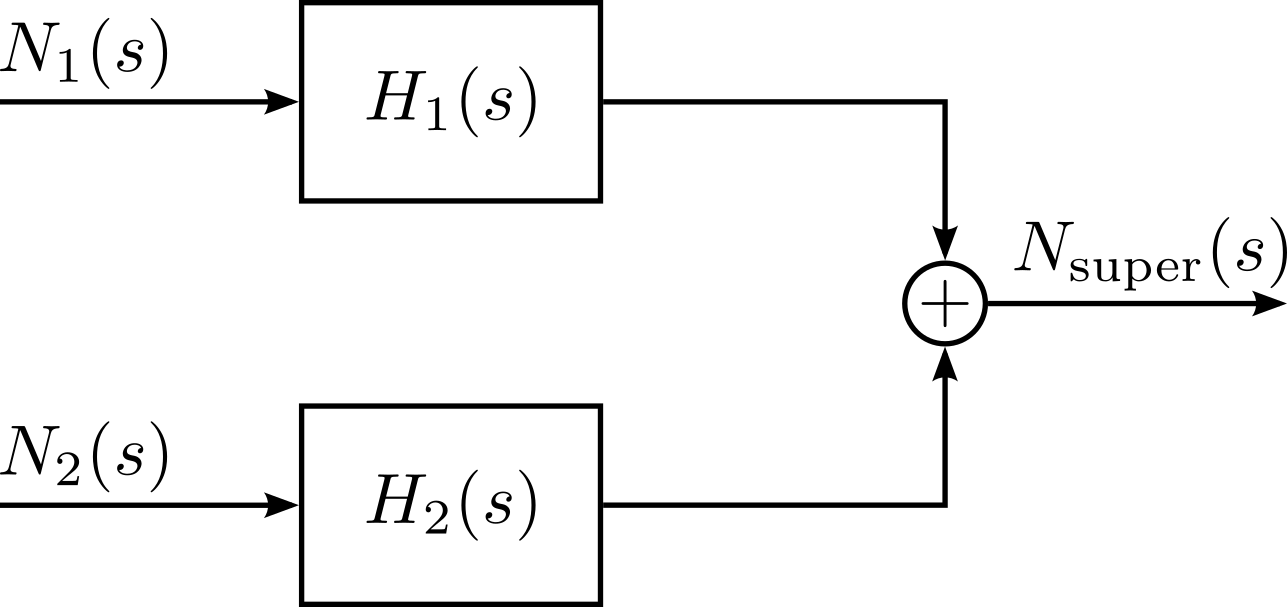
\includegraphics[width=64mm]{figures/complementary_filter}
	\caption{2-sensor blending using complementary filters}
	\label{fig:complementary_filter}
\end{figure}
As shown in the figure, the resultant ``super sensor'' readout has a super sensor noise $N_\mathrm{super}(s)$, and it's given by
\begin{equation}
	N_\mathrm{super}(s) = H_1(s)N_1(s) + H_2(s)N_2(s)\,.
\end{equation}
Note that we omitted the common signal that the sensors are measuring and simply focus on the noises.
Since we expect the super sensor readout to contain the original common signal, the  filters $H_1(s)$ and $H_2(s)$ must be complementary, as in
\begin{equation}
	H_1(s) + H_2(s) = 1\,.
\end{equation}
Alternatively, we can express the second filter $H_2(s)$ as $1-H_1(s)$, and so the super sensor noise is a function of one filter,
\begin{equation}
	N_\mathrm{super}(s; H_1(s)) = H_1(s)N_1(s) + \left[1-H_1(s)\right]N_2(s)\,.
\end{equation}
The amplitude spectral density of the super sensor noise is then
\begin{equation}
	\hat{N}_\mathrm{super}(f; H_1(s)) = \left[\left\lvert H_1(s) \right\rvert^2\hat{N}_1^2(f) + \left\lvert 1-H_1(s) \right\rvert^2\hat{N}_2^2(f)\right]^\frac{1}{2}\,,
\end{equation}
where $\hat{N}(s)$ denotes the amplitude spectral densities.
And here, clearly the goal is the design $H_1(s)$ such that some function $J$ of $\hat{N}_\mathrm{super}(f)$ is minimized.
The problem is stated as follow
\begin{equation}
	\minimize_{H_1(s)\in\mathcal{S}} J\mleft(\hat{N}_\mathrm{super}\mleft(f; H_1(s)\mright)\mright)\,,
	\label{eqn:cost_function_complementary_filter}
\end{equation}
where $J$ is some cost function and $\mathcal{S}$ is the set of proper transfer functions.
We didn't specify the cost function $J$ because this is a user-defined objective.
One of the typical choices of $J$ would be the (weighted) 2-norm \cite{norms_for_signals_and_systems}, which is equivalent to expected RMS of the weighted super sensor noise, i.e.
\begin{equation}
	J_2\mleft(H_1(s)\mright) = \left[\int_{-\infty}^\infty \, \hat{N}_\mathrm{super}\mleft(f;H_1(s)\mright)^2 w(f)^2\, df\right]^\frac{1}{2}\,,
	\label{eqn:cost_function_super_sensor_noise_rms}
\end{equation}
where, again, $w(f)$ is some specified weighting function according to specific requirements of the sensor.
Another typical choice of $J$ would be the (weighted) $\infty$-norm \cite{norms_for_signals_and_systems}, peak of the weighted spectral density of the super sensor noise, i.e.
\begin{equation}
	J_\infty\mleft(H_1(s)\mright) = \sup_{f} \left(\hat{N}_\mathrm{super}\mleft(f;H_1(s)\mright)w(f) \right) \,,
\end{equation}
where $\sup()$ denotes the supremum and $w(f)$ in this case would be the inverse of the frequency dependent specification of the sensor noise.
With all that said, these optimization problem defined by Eqn.~\eqref{eqn:cost_function_complementary_filter} may not be easy to solve, as parameterizing the transfer function space $\mathcal{S}$ is not easy.
Instead, these problems are solved using modern control methods like $\mathcal{H}_2/\mathcal{H}_\infty$ methods \cite{feedback_control_theory}, which is rather involved and will not be discussed here.
In a recent article, sensor correction filters (a type of complementary filter) used in LIGO \cite{low_frequency_vibration_isolation_hua} was reproduced using $\mathcal{H}_\infty$ synthesis using frequency dependent specifications by LIGO \cite{complementary_filters_shaping_using_h_infinity_synthesis}.
Unlike that in \cite{low_frequency_vibration_isolation_hua}, method in \cite{complementary_filters_shaping_using_h_infinity_synthesis} are extremely useful in optimizing IIR filters that is directly implementable to KAGRA's current digital system and therefore should be considered\footnote{This is part of my research actually.}.
However, we will only mention this here and details of these advanced methods will be discussed in the advance method section, i.e. Sec.~\ref{sec:suspension_commissioning_advanced_methods}.

Instead of fancy optimization approaches, we will discuss heuristic methods that were used to design complementary filters in KAGRA.
Here, we will present two methods used previously: 1) Predefined filters \cite{Sekiguchi:2016bmv, Heijningen:2018evm}, and 2) Filter shaping according to sensing noises \cite{low_frequency_optimization_and_performance_of_advanced_virgo_seismic_isolation_system}.
The two methods we discuss here will require a sensor noise measurement or modeling prior.
So be sure to check Sec.~\ref{sec:sensor_noise_measurement} and Sec.~\ref{sec:noise_modeling_baseline}.
Also be sure that those noise spectral densities are available before doing anything related to complementary filters.

Throughout the discussion, we will be referring noise $N_1$ to the seismic noise-coupled LVDT readout noise, see Sec.~\ref{sec:sensor_correction} for why this is the case, and $N_2$ to the geophone noise.
The ASD of the LVDT readout noise is defined as
\begin{equation}
	\hat{N}_1(f) = \left[ \hat{N}_\mathrm{LVDT}(f)^2 + \hat{N}_\mathrm{seismic}(f)^2 \right]^\frac{1}{2}\,,
	\label{eqn:seismic_noise_coupled_lvdt_noise}
\end{equation}
where $\hat{N}_\mathrm{LVDT}(f)$ is the ASD of the LVDT self-noise, which has a $f^{-0.5}$ dependency at low frequency and $f^{0}$ dependency at higher frequencies, and $\hat{N}_\mathrm{seismic}(f)$ is the ASD of the seismic noise.
The ASD of the geophone noise is simply
\begin{equation}
	\hat{N}_2(f) = \hat{N}_\mathrm{geophone}(f)\,,
\end{equation}
where $\hat{N}_\mathrm{geophone}(f)$ is the geophone self-noise that has a $f^{-3.5}$ dependency at low frequency and $f^{-1}$ dependency at higher frequencies.
The amplitude spectral densities of these noises are plotted in Fig.~\ref{fig:sensornoisesforcomplementaryfilter}\footnote{I've altered the seismic noise at frequency $<0.4\,\mathrm{Hz}$ to omit the seismometer noise.}.
\begin{figure}[!h]
	\centering
	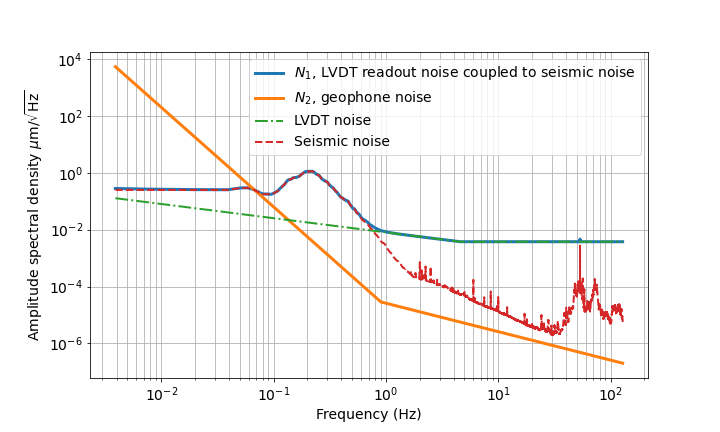
\includegraphics[width=0.7\linewidth]{figures/sensor_noises_for_complementary_filter}
	\caption{Amplitude spectral density of various noises. Blue: LVDT readout noise coupled to seismic noise. Orange: geophone noise. Green dash-dot: LVDT self-noise. Red dashed: Seismic noise from \cite{seismic_noise_kagra}. Note that the seismic noise was measured with seismometers so there're features at higher frequencies that are not really seismic noise, but are sensing artifacts. }
	\label{fig:sensornoisesforcomplementaryfilter}
\end{figure}

\paragraph{Predefined Filters}
In \cite{Sekiguchi:2016bmv} and \cite{Heijningen:2018evm}, sensor fusion using complementary filters to blend LVDTs and geophones at the preisolator stage was briefly discussed.
In \cite{Sekiguchi:2016bmv}, a predefined complementary filter was proposed,
\begin{equation}
	H_1(s;f_b) = \frac{35(2\pi f_b)^4 s^3 + 21(2\pi f_b)^5 s^2 + 7(2\pi f_b)^6 s + (2\pi f_b)^7}{(s+2\pi f_b)^7}\,,
	\label{eqn:complementary_filter_sekiguchi}
\end{equation}
where $f_b$ is the blending frequency at which $\lvert H_1(s)\rvert$ meets $\lvert H_2(s) \rvert$, and $H_2(s)=1-H_1(s)$.
Fig.~\ref{fig:sekiguchicomplementaryfilter} shows an example of Eqn.~\eqref{eqn:complementary_filter_sekiguchi} with blending frequency at $1\,\mathrm{Hz}$.
A simpler one was proposed in \cite{Heijningen:2018evm} but that was for Virgo so we won't mention it here.
\begin{figure}[!h]
	\centering
	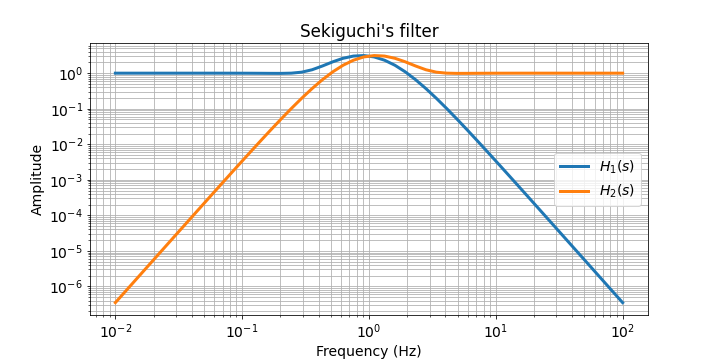
\includegraphics[width=0.7\linewidth]{figures/sekiguchi_complementary_filter}
	\caption{Example complementary filter Eqn.~\eqref{eqn:complementary_filter_sekiguchi} with $f_b=1\,\mathrm{Hz}$.}
	\label{fig:sekiguchicomplementaryfilter}
\end{figure}
The choice of filter shape defined in Eqn.~\eqref{eqn:complementary_filter_sekiguchi} is simple, i.e. the complementary filter $H_2(s)$ is a high-pass filter with fourth-order roll-off at lower frequencies.
The choice of this roll-off is designed to filter out the $f^{-3.5}$ geophone noise\footnote{In this sense, any forth-order high-pass filter should fulfill the purpose. The use of Eqn.~\eqref{eqn:complementary_filter_sekiguchi} is not really justified here. This is why I don't like the predefined filter approach.} as shown in Fig.~\ref{fig:sensornoisesforcomplementaryfilter}.
In \cite{Sekiguchi:2016bmv}, it was also mentioned the sensor noise would be minmized if the choice of blending frequency $f_b$ would be at the cross-over frequency of the two noises\footnote{The statement is vague. What does it mean by minimized? Minimized in what sense? In RMS? Or in peak amplitude?}, i.e. around $70\,\mathrm{mHz}$ in our case.

This method is indeed very simple to implement.
But, there are some caveats and problems to be noted.
First of all, we should note that this method is by definition suboptimal since the shape of the filter defined in Eqn.~\eqref{eqn:complementary_filter_sekiguchi} is hardly justified.
For example, what happens if we switched sensors, say, from geophones to accelerometers?
The noise profile would completely changed and so we might need a different roll-off for the accelerometer.
In this sense, having a predefined filter is not really general enough.
Also, we must note that there will be noise amplification around the blending frequency as shown in Fig.~\ref{fig:sekiguchicomplementaryfilter}.
So, in some extreme case, we might get worsened noise RMS/peak magnitude if the blending frequency is not placed properly.
Also, it's worth pointing out that the low-pass filter has a forth-order roll-off at high frequencies as well.
According to the design logic in \cite{Sekiguchi:2016bmv}, since the LVDT noise has a $f^{0}$ frequency dependency at higher frequencies, it's only required to have a first-order roll-off.
This would mean that the filter is a bit overkilled for the purpose of filtering LVDT noise.
So, why not design a complementary filter that composes of a first-order low-pass and a forth-order high-pass?
In this case, we might even get lower noise amplification at the blending frequency.
Nevertheless, what about the seismic noise coupling we see in the LVDT readout?
Shouldn't we design the complementary filter to account for the microseism around $200\,\mathrm{mHz}$?

\paragraph{Filter shaping according to sensing noises}
This brings us to the method used in \cite{low_frequency_optimization_and_performance_of_advanced_virgo_seismic_isolation_system}, filter shaping according to the sensor noise.
This method was brought to KAGRA by suspension experts in Virgo.
However, this method is closed-source and is not well known in KAGRA, even if those filters have been installed to the Type-A suspensions.
Therefore, here, I would like to reverse-engineer this approach.
I have used optimization methods to optimize complementary filters by minimizing various cost functions including the expected RMS of super sensor noise, i.e. Eqn.~\eqref{eqn:cost_function_super_sensor_noise_rms}, and the optimized filters strongly resembles those filters designed by this method.
So, personally, I think this is a slightly superior method compared to the predefined filter method in \cite{Sekiguchi:2016bmv, Heijningen:2018evm}.
To use this method, it's required to have good knowledge in filter shaping.
And so, this method can only be used by experts and it's likely to be irreproducible.
This is the downside of this method.

This method relies on designing a general filter/transfer function
\begin{equation}
	H_1(s;\theta_{H_1}) = \frac{\prod_i^{n_z}\left( s/z_i+1\right)}{\prod_j^{n_p} \left(s/p_j+1\right)}\frac{\prod_m^{n_{cz}} \left( \frac{1}{\omega_m^2}s^2 + \frac{1}{q_m \omega_m}s + 1 \right)}{\prod_n^{n_{cp}} \left(\frac{1}{\Omega_n^2}s^2 + \frac{1}{Q_n \Omega_n}s + 1 \right)}\,,
	\label{eqn:complementary_filter_general}
\end{equation}
where, $\theta_{H_1}$ are the design parameters $\left[z_i,p_j,\omega_m,q_m,\Omega_n,Q_n,n_z,n_p,n_{cz},n_{zp}\right]^T$, $z_i,p_j\in\mathbb{R}^+$ are the angular frequencies of the simple zeros and simple poles, $\omega_m,\Omega_n\in\mathbb{R}^+$ are the angular frequencies of the complex zeros and complex poles\footnote{Here, we defined complex zeros and poles as a second-order section in the numerator and the denominator respectively.}, $q_m,Q_n\in\mathbb{R}^+$ are the quality factors of the complex zeros and complex poles, and $n_z$, $n_p$, $n_{cz}$, and $n_{cp}$ are the number of zeros, poles, complex zeros, and complex poles, respectively.
Here, we have four types of elements, simple zeros $(s/z_i+1)$, simple poles $(\frac{1}{s/p_i+1})$, complex zeros $(\frac{1}{\omega_m}s^2+\frac{1}{q_m\omega_m}s+1)$, and complex poles $(\frac{1}{\frac{1}{\Omega_m}s^2+\frac{1}{Q_m\Omega_m}s+1})$, and the filter is defined as the produce of these elements.
The effect of these element in the magnitude response of the filter is well understood.
A simple zero will increase the slope of the magnitude response by 1 order per decade starting from the location of the zero $z_i$, while a simple pole will decrease the slope at the pole $p_j$ instead.
A complex zero will create a notch at the complex zero frequency $\omega_m$ and will increase the slope of the magnitude response by 2 orders per decade.
All these features combined can make any filter shape.
So unlike Eqn.~\eqref{eqn:complementary_filter_sekiguchi}, Eqn.~\eqref{eqn:complementary_filter_general} is maximally flexible.
This is also the reason why it can be hard to design.

\begin{figure}[!h]
	\centering
	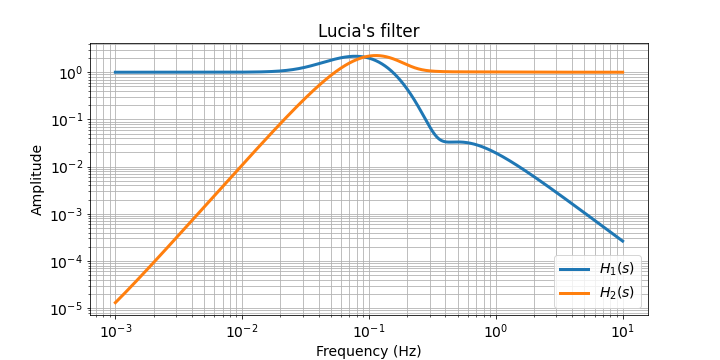
\includegraphics[width=0.7\linewidth]{figures/lucia_complementary_filter}
	\caption{Example complementary filter designed using method in \cite{low_frequency_optimization_and_performance_of_advanced_virgo_seismic_isolation_system}.}
	\label{fig:luciacomplementaryfilter}
\end{figure}
Fig.~\ref{fig:luciacomplementaryfilter} shows an example filter from \cite{low_frequency_optimization_and_performance_of_advanced_virgo_seismic_isolation_system}.
This filter may not be designed for KAGRA's sensors, but the concept is transferable.
Here, we will first qualitatively describe what is the rationale behind the design.
And then, we will do a break down of the transfer function expression of the filters in Fig.~\ref{fig:luciacomplementaryfilter} and attempt to reconstruct a filter like that.

The idea of this design goes as follows.
For the low-pass filter $H_1(s)$, we would like a $2^\mathrm{nd}$-order roll-off at high frequencies.
As for the high-pass $H_2(s)$, we are looking for a $3^\mathrm{rd}$-order roll-off at lower frequencies.
These roll-off orders are designed according to the noise amplitude spectral densities $\hat{N}_1(f)$ and $\hat{N}_2(f)$.
We can choose the roll-off order based on arguments in \cite{Sekiguchi:2016bmv}.
For example, if we expect the noise $\hat{N}_2(f)$ to have a $f^{-3.5}$ frequency dependency at lower frequencies, then the filter $H_2(s)$ should have at least that order of roll-off, i.e. $4^\mathrm{th}$-order roll-off.
Alternatively, the relative order between $\hat{N}_1(f)$ and $\hat{N}_2(f)$ is considered.
For example, if $\hat{N}_1(f)$ has a frequency dependency of $f^{-0.5}$ at lower frequencies and $\hat{N}_2(f)$ has a frequency dependency of $f^{-3.5}$ at lower frequency, the relative order is 3.
This means a $3^\mathrm{rd}$-order roll-off for $H_2(s)$ is sufficient so the noise $\hat{N}_2(f)$ not over-suppressed.
This is more optimal since over-suppressing would necessarily mean more noise-amplification around the blending frequency (See Bode's sensitivity integral for more details \cite{wiki:bode's_sensitivity_integral}.).
Like-wise, we can choose the roll-off for the low-pass following the same argument.
But in this case, $2^\mathrm{nd}$-order was chosen for whatever reason.
Another main difference between filters in Fig.~\ref{fig:luciacomplementaryfilter} and Fig.~\ref{fig:sekiguchicomplementaryfilter} is the ``notch'' in the low-pass filter at around $0.4\,\mathrm{Hz}$.
The low-pass filter is designed to have a higher-order roll-off around $0.1$ to $0.4\,\mathrm{Hz}$ for the purpose of filtering out the microseism around $0.2\,\mathrm{Hz}$.
The (secondary) microseism \cite{wiki:microseism} is a bump at around $0.2\,\mathrm{Hz}$ in the seismic noise spectrum, which is obviously visible in $N_1$ (blue curve) in Fig.~\ref{fig:sensornoisesforcomplementaryfilter}.
To prevent over-filtering, the low-pass returns to the $2^\mathrm{nd}$-order filtering at higher frequencies.
With these design features, the shapes of the low-pass and high-pass are roughly fixed except the blending frequency.
The blending frequency is the chosen to be high enough such that the inertial sensing noise at lower frequencies does not compromise the expected RMS of the super sensor noise.
Again, this will be around the cross-over frequency of the two sensing noises.

Now, let's reverse-engineer the filter shown in Fig.~\ref{fig:luciacomplementaryfilter} and see if we can design something similar.
The low-pass filter\footnote{I was given the filter by Lucia herself a few years ago.} shown in figure is expressed as
\begin{equation}
	H_1(s) = \frac{\left(\frac{1}{\omega_1^2}s^2+\frac{1}{q_1\omega_1}s+1\right)\left(\frac{1}{\omega_2^2}s^2+\frac{1}{q_2\omega_2}s+1\right)\left(\frac{1}{\omega_3^2}s^2+\frac{1}{q_3\omega_3}s+1\right)}{(s/p_1+1)^5(s/p_2+1)^3}\,,
	\label{eqn:complementary_low-pass_filter_lucia}
\end{equation}
where $\frac{p_1}{2\pi} = 0.12\,\mathrm{Hz}$, $\frac{p_2}{2\pi} = 0.25\,\mathrm{Hz}$, $\frac{\omega_1}{2\pi}=\frac{\omega_2}{2\pi} = 0.35\,\mathrm{Hz}$, $\frac{\omega_3}{2\pi} = 0.031272069\,\mathrm{Hz}$, $q_1 = 2$, $q_2 = 1.1$, and $q_3 = 0.64417749$.
From these values, we immediately see part of the story behind the design: the poles and the first two complex zeros are designed values while the third complex zero is passively derived numerically.
The reason why we cannot assign all parameters is because we want the complementary filter
$H_2(s)=1-H_1(s)$ to be a third-order high-pass filter.
This necessarily means that $H_2(s)$ must have 3 zeros at $0\,\mathrm{Hz}$ (or negligibly low frequency), i.e. $H_2(s) = \frac{s^3\dots}{\dots}$, and no poles between the blending frequency and $0\,\mathrm{Hz}$.
While $H_2(s) = 1-H_1(s) = \frac{\dots}{\left(s/p_1+1\right)^5\left(s/p_2+1\right)^3}$ that $H_1(s)$ and $H_2(s)$ to share the same poles, this guarantees that there will be no poles in $H_2(s)$ before the blending frequency, which will be slightly before $\frac{p_1}{2\pi}$.

Now, let's write $H_1(s)$ in a more general transfer function form
\begin{equation}
	H_1(s) = \frac{B(s)}{A(s)} = \frac{\sum_{i=0}^6 b_is^i}{\sum_{j=0}^8 a_js^j}\,,
	\label{eqn:complementary_low-pass_filter_lucia_polynomial}
\end{equation}
where $B(s)$ and $A(s)$ are the numerator and denominator polynomials of the $H_1(s)$ transfer function and $b_i$ and $a_j$ are the polynomial coefficients.
And, as for $H_2(s)$, it becomes
\begin{equation}
	H_2(s) = 1-H_1(s) = \frac{\sum_{j=0}^8 a_js^j - \sum_{i=0}^6 b_is^i}{\sum_{j=0}^8 a_j s^j}\,.
\end{equation}
So it follows that $a_2-b_2=a_1-b_1=a_0-b_0=0$ are the requirements, if we want $H_2(s) = \frac{s^3\dots}{\dots}$, i.e. a $3^\mathrm{rd}$-order high-pass filter.
Inspecting Eqn.~\eqref{eqn:complementary_low-pass_filter_lucia}, we see that $a_0=b_0=1$ so $a_0-b_0=0$ is automatically satisfied.
This means what we still need to engineer $b_2$ and $b_1$ so they equals to $a_2$ and $a_1$ respectively.
This explains why there are two passively derived values, $\omega_3$ and $q_3$, in Eqn.~\eqref{eqn:complementary_low-pass_filter_lucia}.
Let's assume that we designed other parameters (we shall explain this later) except $\omega_3$ and $q_3$.
Now, we just need to solve for them algebraically.
Plugging in $\frac{p_1}{2\pi} = 0.12\,\mathrm{Hz}$, $\frac{p_2}{2\pi} = 0.25\,\mathrm{Hz}$ into $A(s) = (s/p_1+1)^5(s/p_2+1)^3$, we get
\begin{equation}
	a_2=31.47148543 \quad\text{and}\quad a_1=8.54131528\,.
\end{equation}
Expanding $B(s)=\left(\frac{1}{\omega_1^2}s^2+\frac{1}{q_1\omega_1}s+1\right)\left(\frac{1}{\omega_2^2}s^2+\frac{1}{q_2\omega_2}s+1\right)\left(\frac{1}{\omega_3^2}s^2+\frac{1}{q_3\omega_3}s+1\right)$,
we get
\begin{equation}
	b_2 = \frac{1}{\omega_1^2} + \frac{1}{\omega_2^2} + \frac{1}{\omega_3^2} + \frac{1}{q_1\omega_1 q_2\omega_2} + \frac{1}{q_1\omega_1 q_3\omega_3} + \frac{1}{q_2\omega_2 q_3\omega_3}\,,
	\label{eqn:b_2_unsolved}
\end{equation}
and
\begin{equation}
	b_1 = \frac{1}{q_1\omega_1}+\frac{1}{q_2\omega_3}+\frac{1}{q_3\omega_3}\,.
\end{equation}
By equating $b_1=a_1=8.54131528$ and substituting $\frac{\omega_1}{2\pi}=\frac{\omega_2}{2\pi} = 0.35\,\mathrm{Hz}$, $q_1 = 2$, and $q_2 = 1.1$, we get
\begin{equation}
	\frac{1}{q_3\omega_3} = 7.9005615330066545\,.
	\label{eqn:1_over_q3_omega3}
\end{equation}
Substituting Eqn.~\eqref{eqn:1_over_q3_omega3} $\frac{\omega_1}{2\pi}=\frac{\omega_2}{2\pi} = 0.35\,\mathrm{Hz}$, $q_1 = 2$, $q_2 = 1.1$, and $b_2=a_2=31.47148543$ into \eqref{eqn:b_2_unsolved} and solve for $\omega_3$,
we get
\begin{equation}
	\begin{split}
		\frac{1}{\omega_3^2} &= 25.901625838545005\\
		\frac{\omega_3}{2\pi} &= 0.03127206923221885\,\mathrm{Hz}\,,
	\end{split} 
\end{equation}
where we of course reject the negative values corresponds to an unstable zero.
This matches the initial statement where we say $\frac{\omega_3}{2\pi} = 0.031272069\,\mathrm{Hz}$ is a derived value.
Solving for $q_3$, and not surprisingly, we get
\begin{equation}
	\begin{split}
		q_3 &= \frac{1}{7.900\dots\omega_3}\\
		&= 0.6441775018514415
	\end{split}
\end{equation}
which also equals the inital statement where we say $q_3 = 0.64417749$ is a derived value.

Now, let's see how are the other parameters decided.
First of all, let's remind ourselves what are the requirements of this filter.
The low-pass filter $H_1(s)$ has to have second-order roll-off at higher frequencies.
This means that the order of the denominator polynomial $A(s)$ has to at least 2.
We said that the high-pass filter $H_2(s)$ has to have third-order roll-off.
While $H_2(s) = 1-H_1(s) = \frac{A(s)-B(s)}{A(s)}$, and the order of $B(s)$ is less than that of $A(s)$, the order of $A(s)$ must be at least 3.
Now, as mentioned we need to have 2 derived parameters in $B(s)$ so the order of $B(s)$ is at least 2.
Since $H_1(s$ is designed to have second-order roll-off, the relative order between $B(s)$ and $A(s)$ must be 2, so now the order of $A(s)$ must be at least 4.
Now, this is the tricky part.
By inspecting the $N_1$ noise in Fig.~\ref{fig:sensornoisesforcomplementaryfilter}, we see that the microseism is roughly 2 orders of magnitude higher than that of the geophone noise $N_2$.
While the microseism noise spans around half a decade, to completely suppress it would require a $4^\mathrm{th}$-order roll-off before the microseism.
In other words, we would require 4 additional order in $A(s)$ to suppress this, and also 4 addition order in $B(s)$ to cancel the high-order roll-off so to retain a $2^\mathrm{nd}$ order roll-off at higher frequencies.
These constrain $A(s)$ to be an $>8^\mathrm{th}$-order polynomial and $B(s)$ to be an $>6^\mathrm{th}$-order polynomial.
This justifies the form as shown in Eqn.~\eqref{eqn:complementary_low-pass_filter_lucia_polynomial}.
Converting from Eqn.~\eqref{eqn:complementary_low-pass_filter_lucia_polynomial} to Eqn.~\eqref{eqn:complementary_low-pass_filter_lucia} is purely a designer's choice as it's free to construct the polynomials using either simple zeros/poles or complex zeros/poles.
However, it's important to set the frequencies of the zeros and poles according to the purpose.
Here, as we would like to filter out the microseism, $p_1$ was chosen to be at $0.12\,\mathrm{Hz}$ so the low-pass roll-offed before the microseism frequency.
The choice of the order $p_1$ is $5$ which would be arguable as it might the roll-off might be reduced to $3^\mathrm{rd}$-order if one of the frequencies of the complex zeros is lower than that of $p_1$, which is actually the case.
The frequency of $p_2$ is chosen to be $0.25\,\mathrm{Hz}$, which is not that important so long as it's
in between the frequencies of the two complex zeros, which is $0.35\,\mathrm{Hz}$.
The frequencies of the complex zeros are chosen to be slightly higher than that of the microseism so the low-pass filter returns to a the final designed $2^\mathrm{nd}$-order roll-off.
The Q factors for the first and second are tunable parameters so to finely adjust the blending frequency as well as the suppression needed at the complex zeros frequencies.
The ended up irrelevant as they were set to very low.
At last, as mentioned, the frequency and the Q factor of the final complex zero was passive determined by requiring the high-pass filter $H_2(s)$ to have $3^\mathrm{rd}$-order roll-off.
This is how a complementary filter is designed and justified.

Now, this will become very tedious but there's a resolution.
As mentioned before, if we use optimization approach to minimize the super sensor noise by optimize an arbitrary $H_1(s)$ that has a $6^\mathrm{th}$-order numerator and $8^\mathrm{th}$-order numerator, then the result will be very similar to that shown in Fig.~\ref{fig:luciacomplementaryfilter}.
And, it'll be arguably better because it's optimized instead of tuned.
But let's not overcrowd this section and left this discussion to a later section (Sec.~\ref{sec:suspension_commissioning_advanced_methods}).
For a sneak peek, please see \cite{srm_inertial_damping, discussion_on_vis_inertial_sensor} for a very preliminary implementation of these optimization methods.

\subsubsection{Sensor correction \label{sec:sensor_correction}}
Displacement sensors on the suspensions are typically relative displacement sensors that measure differential motion.
Some displacement sensors are mounted on an non-suspended structure so the they measure the differential motion between the suspension and the ground.
Example sensors are the LVDTs at the preisolator stage and the optical levers measuring the longitudinal motion of the optics.
These sensors, in addition to the self sensor noise, are coupled to seismic noise, so the sensing noise is sum of the sensor self noise and the seismic noise.
This is why we set the sensor noise in Eqn.~\eqref{eqn:seismic_noise_coupled_lvdt_noise} as a quadrature sum of LVDT noise and seismic noise.
Sensors that are coupled to seismic noise cannot be used for active seismic isolation as seismic noise would be re-introduced as control noise.
To maximize the control potential, on top of sensor blending using complementary filter (Sec.~\eqref{sec:complementary_filter}), we can artificially remove the seismic noise coupling from those seismic noise-coupled sensors by ``sensor correction''.

Sensor correction is a technique first used by LIGO to reduce seismic noise coupling from the relative displacement sensors \cite{Matichard_2015}.
\begin{figure}
	\centering
	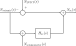
\includegraphics[width=76mm]{figures/sensor_correction}
	\caption{Sensor correction block diagram.}
	\label{fig:sensorcorrection}
\end{figure}

\subsubsection{Examples \label{sec:sensor_fusion_examples}}